% Тип документа
\documentclass[a4paper,12pt]{extarticle}

% Шрифты, кодировки, символьные таблицы, переносы
\usepackage{cmap}
\usepackage[T2A]{fontenc}
\usepackage[utf8x]{inputenc}
\usepackage[russian]{babel}

% Это пакет -- хитрый пакет, он нужен но не нужен
\usepackage[mode=buildnew]{standalone}

\usepackage
	{
		% Дополнения Американского математического общества (AMS)
		amssymb,
		amsfonts,
		amsmath,
		amsthm,
		physics,
		% misccorr,
		% 
		% Графики и рисунки
		wrapfig,
		graphicx,
		subcaption,
		float,
		tikz,
		tikz-3dplot,
		caption,
		csvsimple,
		color,
		booktabs,
		pgfplots,
		pgfplotstable,
		geometry,
		% 
		% Таблицы, списки
		array,
		makecell,
		multirow,
		indentfirst,
		%
		% Интегралы и прочие обозначения
		ulem,
		esint,
		esdiff,
		% 
		% Колонтитулы
		fancyhdr,
	}  

\usepackage{xcolor}
\usepackage{hyperref}

 % Цвета для гиперссылок
\definecolor{linkcolor}{HTML}{000000} % цвет ссылок
\definecolor{urlcolor}{HTML}{799B03} % цвет гиперссылок
 
\hypersetup{pdfstartview=FitH,  linkcolor=linkcolor,urlcolor=urlcolor, colorlinks=true}
% Обводка текста в TikZ
\usepackage[outline]{contour}

% Увеличенный межстрочный интервал, французские пробелы
\linespread{1.3} 
\frenchspacing 

 
\usetikzlibrary
	{
		decorations.pathreplacing,
		decorations.pathmorphing,
		patterns,
		calc,
		scopes,
		arrows,
		fadings,
		through,
		shapes.misc,
		arrows.meta,
		3d,
		quotes,
		angles,
		babel
	}


\tikzset{
	force/.style=	{
		>=latex,
		draw=blue,
		fill=blue,
				 	}, 
	%				 	
	axis/.style=	{
		densely dashed,
		blue,
		line width=1pt,
		font=\small,
					},
	%
	th/.style=	{
		line width=1pt},
	%
	acceleration/.style={
		>=open triangle 60,
		draw=magenta,
		fill=magenta,
					},
	%
	inforce/.style=	{
		force,
		double equal sign distance=2pt,
					},
	%
	interface/.style={
		pattern = north east lines, 
		draw    = none, 
		pattern color=gray!60,
					},
	cross/.style=	{
		cross out, 
		draw=black, 
		minimum size=2*(#1-\pgflinewidth), 
		inner sep=0pt, outer sep=0pt,
					},
	%
	cargo/.style=	{
		rectangle, 
		fill=black!70, 
		inner sep=2.5mm,
					},
	%
	caption/.style= {
		midway,
		fill=white!20, 
		opacity=0.9
					},
	%
	}

\newenvironment{tikzpict}
    {
	    \begin{figure}[htbp]
		\centering
		\begin{tikzpicture}
    }
    { 
		\end{tikzpicture}
		% \caption{caption}
		% \label{fig:label}
		\end{figure}
    }


\newcommand{\vbLabel}[3]{\draw ($(#1,#2)+(0,5pt)$) -- ($(#1,#2)-(0,5pt)$) node[below]{#3}}
\newcommand{\vaLabel}[3]{\draw ($(#1,#2)+(0,5pt)$) node[above]{#3} -- ($(#1,#2)-(0,5pt)$) }

\newcommand{\hrLabel}[3]{\draw ($(#1,#2)+(5pt,0)$) -- ($(#1,#2)-(5pt,0)$) node[right, xshift=1em]{#3}}
\newcommand{\hlLabel}[3]{\draw ($(#1,#2)+(5pt,0)$) node[left, xshift=-1em]{#3} -- ($(#1,#2)-(5pt,0)$) }



\newcommand\zi{^{\,*}_i}
\newcommand\sumn{\sum_{i=1}^{N}}

\tikzset{
	coordsys/.style={scale=1.8,x={(1.1cm,-0cm)},y={(0.5cm,1cm)}, z={(0cm,0.8cm)}},
	coordsys/.style={scale=1.5,x={(0cm,0cm)},y={(1cm,0cm)}, z={(0cm,1cm)}}, 
	coordsys/.style={scale=1.5,x={(1cm,0cm)},y={(0cm,1cm)}, z={(0cm,0cm)}}, 
}

\usepgfplotslibrary{units}


% Draw line annotation
% Input:
%   #1 Line offset (optional)
%   #2 Line angle
%   #3 Line length
%   #5 Line label
% Example:
%   \lineann[1]{30}{2}{$L_1$}

\newcommand{\lineann}[4][0.5]{%
    \begin{scope}[rotate=#2, blue,inner sep=2pt, ]
        \draw[dashed, blue!40] (0,0) -- +(0,#1)
            node [coordinate, near end] (a) {};
        \draw[dashed, blue!40] (#3,0) -- +(0,#1)
            node [coordinate, near end] (b) {};
        \draw[|<->|] (a) -- node[fill=white, scale=0.8] {#4} (b);
    \end{scope}
}

\newcommand{\lineannn}[4][0.5]{%
    \begin{scope}[rotate=#2, blue,inner sep=2pt, ]
        \draw[dashed, blue!40] (0,0) -- +(0,#1)
            node [coordinate, near end] (a) {};
        \draw[dashed, blue!40] (#3,0) -- +(0,#1)
            node [coordinate, near end] (b) {};
        % \draw[color=white, color=blue] (a) -- node[fill=white, scale=0.8] {#4} (b);
        \draw[->|] (a)++(-0.3,0) -- (a);
        \draw[->|] (b)++(0.3,0) coordinate (xx) -- (b);
        \draw (xx) node[fill=white, scale=0.8, right] {#4};
    \end{scope}
}

% Круговая стрелка относительно центра (дуга из центра)
\tikzset{
  pics/carc/.style args={#1:#2:#3}{
    code={
      \draw[pic actions] (#1:#3) arc(#1:#2:#3);
    }
  },
  dash/.style={
  	dash pattern=on 5mm off 5mm
  }
}

% Среднее <#1>
\newcommand{\mean}[1]{\langle#1\rangle}

\pgfplotsset{
    % most recent feature set of pgfplots
    compat=newest,
}

% const прямым шрифтом
\newcommand\ct[1]{\text{\rmfamily\upshape #1}}
\newcommand*{\const}{\ct{const}}


\usepackage[europeanresistors,americaninductors]{circuitikz}

% Style to select only points from #1 to #2 (inclusive)
\pgfplotsset{select/.style 2 args={
    x filter/.code={
        \ifnum\coordindex<#1\def\pgfmathresult{}\fi
        \ifnum\coordindex>#2\def\pgfmathresult{}\fi
    }
}}


\usepackage{array}
\usepackage{pstool}


%%%%%%%%%%%%%%%%%%%%%%%%%%%%%%%%%%%%%%%%%%%%%%%%%
\makeatletter
\newif\if@gather@prefix 
\preto\place@tag@gather{% 
  \if@gather@prefix\iftagsleft@ 
    \kern-\gdisplaywidth@ 
    \rlap{\gather@prefix}% 
    \kern\gdisplaywidth@ 
  \fi\fi 
} 
\appto\place@tag@gather{% 
  \if@gather@prefix\iftagsleft@\else 
    \kern-\displaywidth 
    \rlap{\gather@prefix}% 
    \kern\displaywidth 
  \fi\fi 
  \global\@gather@prefixfalse 
} 
\preto\place@tag{% 
  \if@gather@prefix\iftagsleft@ 
    \kern-\gdisplaywidth@ 
    \rlap{\gather@prefix}% 
    \kern\displaywidth@ 
  \fi\fi 
} 
\appto\place@tag{% 
  \if@gather@prefix\iftagsleft@\else 
    \kern-\displaywidth 
    \rlap{\gather@prefix}% 
    \kern\displaywidth 
  \fi\fi 
  \global\@gather@prefixfalse 
} 
\newcommand*{\beforetext}[1]{% 
  \ifmeasuring@\else
  \gdef\gather@prefix{#1}% 
  \global\@gather@prefixtrue 
  \fi
} 
\makeatother
%%%%%%%%%%%%%%%%%%%%%%%%%%%%%%%%%%%%%%%%%%%%%%%%%

\geometry		
	{
		left			=	2cm,
		right 			=	2cm,
		top 			=	3cm,
		bottom 			=	3cm,
		bindingoffset	=	0cm
	}

%%%%%%%%%%%%%%%%%%%%%%%%%%%%%%%%%%%%%%%%%%%%%%%%%%%%%%%%%%%%%%%%%%%%%%%%%%%%%%%



	%применим колонтитул к стилю страницы
\pagestyle{fancy} 
	%очистим "шапку" страницы
\fancyhead{} 
	%слева сверху на четных и справа на нечетных
\fancyhead[R]{\labauthors} 
	%справа сверху на четных и слева на нечетных
\fancyhead[L]{Отчёт по лабораторной работе №\labnumber} 
	%очистим "подвал" страницы
\fancyfoot{} 
	% номер страницы в нижнем колинтуле в центре
\fancyfoot[C]{\thepage} 

%%%%%%%%%%%%%%%%%%%%%%%%%%%%%%%%%%%%%%%%%%%%%%%%%%%%%%%%%%%%%%%%%%%%%%%%%%%%%%%

\renewcommand{\contentsname}{Оглавление}

\usepackage{tocloft}
% \renewcommand{\cftpartleader}{\cftdotfill{\cftdotsep}} % for parts
% \renewcommand{\cftsectiondotsep}{\cftdotsep}% Chapters should use dots in ToC
\renewcommand{\cftsecleader}{\cftdotfill{\cftdotsep}}
%\renewcommand{\cftsecleader}{\cftdotfill{\cftdotsep}} % for sections, if you really want! (It is default in report and book class (So you may not need it).
% ---------
% \newcommand{\cftchapaftersnum}{.}%
% \usepackage{titlesec}
% \titlelabel{\thetitle.\quad}
\usepackage{secdot}
\sectiondot{subsection}



% \mathtoolsset{showonlyrefs=true}
\newcommand\Smat{\hat { \mathbf { S } }}
\let\tempint\int
\renewcommand{\int}{\tempint\limits}
\DeclareMathOperator{\Div}{div}
\DeclareMathOperator{\Rot}{rot}
\DeclareMathOperator{\Grad}{grad}
\renewcommand{\phi}{\varphi}

\begin{document}

\def\labauthors{Виноградов И.Д., Шиков А.П.}
\def\labgroup{430}
\def\labnumber{3}
\def\labtheme{Измерение dремени жизни и диффузионной длины неосновных носителей заряда в полупроводниках}
\begin{titlepage}

\begin{center}

{\small\textsc{Нижегородский государственный университет имени Н.\,И. Лобачевского}}
\vskip 1pt \hrule \vskip 3pt
{\small\textsc{Радиофизический факультет. Кафедра Радиотехники.}}

\vfill

{\Large Отчет по лабораторной работе №\labnumber\vskip 12pt\bfseries \labtheme}
	
\end{center}

\vfill
	
\begin{flushright}
	{Выполнили студенты \labgroup\ группы\\ \labauthors}%\vskip 12pt Принял:\\ Менсов С.\,Н.}
\end{flushright}
	
\vfill
	
\begin{center}
	Нижний Новгород, \the\year
\end{center}

\end{titlepage}



\section*{Введение}

Одна из особенностей полупроводниковых кристаллов состоит в том, что концентрация носителей заряда в полупроводниках
сильно меняется при изменении температуры, освещении, приложении внешних электрических напряжений и т.п. Такое изменение
обусловлено разрывом валентных связей кристаллической решетки полупроводника (рис. \ref{fig:figure1}).
\begin{figure}[H]
	\centering
	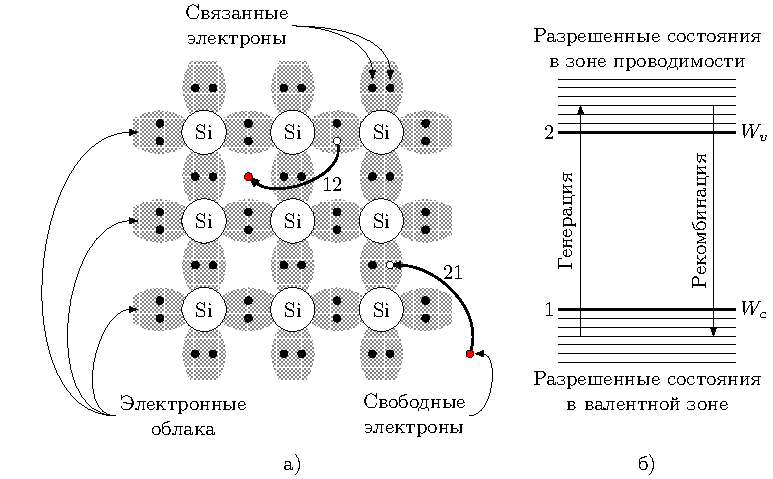
\includegraphics[]{fig/cryst}
	\caption{Схематическое изображение кристаллической решетки кремния (а) и его зонная диаграмма (б).}
	\label{fig:figure1}
\end{figure}

Явление перехода электрона из связанного состояния в валентной зоне в зону проводимости с разрывом валентной связи
называется генерацией. В процессе генерации образуется электрон в зоне проводимости и оборванная валентная связь - дырка
в зоне проводимости. Обратный процесс перехода электрона в валентную зону с восстановлением валентной связи называют
рекомбинацией.

Напомним, что если замкнутая макроскопическая система находится в таком состоянии, в котором для любой ее части
являющейся самой по себе макроскопическим телом, макроскопические величины с большой относительной точностью равны своим
средним значениям, то система находится в состоянии термодинамического равновесия. Даже в условиях
равновесного состояния при температурах отличных от абсолютного нуля в полупроводнике непрерывно происходит процесс
теплового возбуждения электронов из валентной зоны в зону проводимости. Этот процесс уравновешивается рекомбинацией
электронов из зоны проводимости и дырок из валентной зоны.

При наличии внешних воздействий на полупроводник к тепловым переходам добавляются переходы нетепловой природы, и при
этом частота обратных переходов тоже изменяется. Состояние полупроводника в этих условиях является термодинамически
неравновесным.

Лабораторная работа посвящена исследованию нескольких характеристик неравновесного электронно-дырочного газа -- времени
жизни и диффузионной длины неосновных носителей заряда.

\section*{Теоретическая часть}
\section{Уравнения непрерывности}

Уравнение непрерывности описывает процесс изменения плотности заряда $\rho$ в полупроводниковых структурах за счет
перемещения электронов и дырок в пространстве, характеризующегося плотностью тока $\vec{j}$:

\begin{equation}
	\label{eq1}
	\frac{\partial \rho}{\partial t}=-\operatorname{div} \vec{j}
\end{equation}

Следует отметить, что кроме подвижных электронов и дырок в полупроводнике имеются неподвижные заряженные объекты -
ионизованные атомы примеси, т.е. ионы доноров и акцепторов, а также заряженные дефекты кристаллической решетки. В
уравнении \eqref{eq1} речь идет только о подвижных носителях заряда, в то время как для расчета электрического поля в
полупроводниковых структурах следует учитывать все имеющиеся заряды.

В уравнении непрерывности должны быть добавлены слагаемые, отвечающие за генерацию и рекомбинацию электронно-дырочных пар. Кроме того, поведение
двух типов подвижных носителей заряда более удобно анализировать по отдельности.

\begin{gather}
	\label{eq2}
	\frac{\partial n}{\partial t}=\frac{1}{e} \Div \vec{j}_{n}+G_{n}-R_{n},\\ \nonumber
	\frac{\partial p}{\partial t}=-\frac{1}{e} \Div \vec{j}_{p}+G_{p}-R_{p}
\end{gather}

Здесь $G_n$ и $G_p$ -- скорости генерации электронов и дырок в единице объема, вызываемой внешними воздействиями, $R_n$ и $R_p$ -- скорости рекомбинации электронов и дырок.

\section{Генерация и рекомбинация в прямозонных и непрямозонных полупроводниках}

В процессах генерации и рекомбинации электроннодырочных пар выполняются фундаментальные физические законы - законы
сохранения энергии и квазиимпульса электронов. Рассмотрим процессы, указанные на рисунке \ref{fig:figure1} во введении.
Из закона сохранения энергии следует, что в процессе рекомбинации электрон выделяет избыточную энергию при переходе в
валентную зону и восстановлении связанного состояния (валентной связи). Напротив, в процессе генерации электрон
поглощает энергию извне, что ведет к разрыву валентной связи и переходу электрона в зону проводимости. Как в том, так и
в другом случае энергия может переноситься квантом света, т.е. фотоном или квантом колебаний кристаллической решетки
полупроводника - фононом. Однако не во всех типах полупроводников эти процессы равноправны. Причина этого - различные
условия выполнения закона сохранения импульса при генерации и рекомбинации электронно-дырочных пар.

В прямозонных полупроводниках вершина валентной зоны и дно зоны проводимости находятся в одной точке зоны Бриллюэна
(рис.  \ref{fig:figure2}б), т.е. имеют одну и туже координату по оси абсцисс (один и тот же волновой вектор). Поэтому
квазиимпульс электрона, связанный с волновым вектором ($\vec{p}=\hbar \vec{k}$) при переходе почти не меняется.
Значительное изменение энергии (порядка ширины запрещенной зоны) при очень малом изменении квазиимпульса возможно при
испускании или поглощении кванта электромагнитного излучения, у которого, как известно, импульс мал по величине.

\begin{figure}[h!]
	\centering
	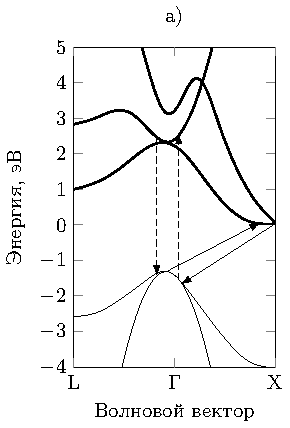
\includegraphics[width = .35\linewidth]{fig/diag}
	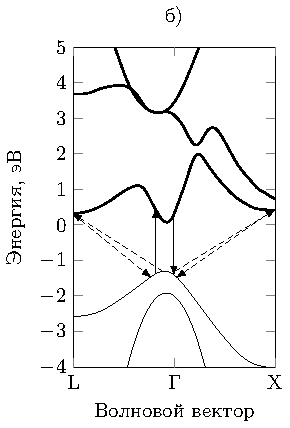
\includegraphics[width = .35\linewidth]{fig/diag2}
	\caption{Зонная диаграмма Si (а) и GaAs (б) полупроводников. 
Стрелками отмечены процессы генерации (1$\to$2) и рекомбинации (2$\to$1) в непрямозонных (а) и прямозонных (б)
полупроводниках.}
	\label{fig:figure2}
\end{figure}
% <img src="Время_жизни_2011_files/1240353c4f_3638373d38_2011-3.png" style="width:147pt;height:162pt;"/>
% 
% рис.  2. 

Напротив, в непрямозонных полупроводниках (рис.  \ref{fig:figure2}а) вершина валентной зоны и дно зоны проводимости
находятся в разных точках зоны Бриллюэна. Поэтому квазиимпульс электрона сильно изменятся при межзонном переходе. Чаще
всего это происходит при испускании или поглощении оптического фонона у которого квазиимпульс велик из-за большой массы
атомов полупроводника, совершающих тепловые колебания. Заметим, что одновременно изменение, как энергии, так и
квазиимпульса электрона при межзонном переходе происходит и при оже-рекомбинации, когда избыточная энергия и
квазиимпульс передаются другому электрону или дырке. Обратным процессом оже-рекомбинации является ударная ионизация.



Поглощение оптического излучения в полупроводнике характеризуется коэффициентом поглощения. В случае, когда энергия
кванта чуть больше ширины запрещенной зоны, т.е. вблизи края фундаментального поглощения полупроводника, коэффициент
поглощения определяется, как 
\begin{gather}
	\label{eq3}
	\alpha \sim\left(h\nu-W_{g}\right)^{\gamma}
\end{gather}
где $h\nu$ - энергия фотона, $W_g$ - ширина запрещенной зоны. Теоретически (в одноэлектронном приближении) $\gamma=\frac12$ для разрешенных
прямых переходов и $\gamma=2$ для непрямых переходов, которые происходят с участием фононов.

Если уровень расположен вблизи середины запрещенной зоны
полупроводника (так называемый глубокий уровень), то вероятность попадания на него как электрона, так и дырки примерно
одинакова. Напротив, если уровень расположен вблизи валентной зоны или зоны проводимости (мелкий уровень), то
вероятности попадания на такой уровень носителей разных знаков существенно различны.

Таким образом, рекомбинационные процессы при наличии глубокого уровня протекают в две стадии: сначала на глубокий
уровень захватывается носитель одного знака, а затем другого. Мелкие уровни не оказывают существенного влияния на
скорость рекомбинации, так как в этом случае скорость рекомбинации будет определяться меньшей из вероятностей попадания
носителей на уровень. При наличии одного глубокого уровня скорость рекомбинации может быть описана на основе теории
Шокли-Рида-Холла

При малых уровнях инжекции, часто используют приближение <<времени жизни>>, основанное на разложении $R(n,p)$ в ряд Тейлора в линейном приближении 
\begin{gather}
	\label{eq6}
	R(n, p)=\left(\frac{\partial R}{\partial n}\right)_{p=n_{0} \atop p=p_{0}} \delta n+\left(\frac{\partial R}{\partial p}\right)_{n=n_{0} \atop p=p_{0}} \delta p
\end{gather}
Введем величины 
\begin{equation*}
	\tau_{n}=\left(\frac{\partial R}{\partial n}\right)_{n=n_{0} \atop p=p_{0}}^{-1}
	\qq{и}
	\tau_{p}=\left(\frac{\partial R}{\partial p}\right)_{n=p_{0} \atop p=p_{0}}^{-1},
\end{equation*}  имеющие размерность времени и характеризующие протяженность интервала существования неосновных носителе заряда от момента генерации до их рекомбинации.

С учетом \eqref{eq6} уравнения непрерывности можно записать в виде
\begin{gather}
	\label{eq7}
	\frac{\partial n}{\partial t}=\frac{1}{e} \Div \vec{j}_{{n}}+G_{n}-\frac{n-n_{0}}{\tau_{n}}\\
	\frac{\partial p}{\partial t}=-\frac{1}{e} \Div \vec{j}_{{p}}+G_{p}-\frac{p-p_{0}}{\tau_{p}}
\end{gather}


\section{Метод измерения времени жизни неосновных носителей заряда}
Как показано в предыдущем разделе для измерения времени жизни и диффузионной длины неосновных носителей заряда
необходимо создать неравновесное состояние электронно-дырочного газа в полупроводниковом кристалле. Сделать это проще
всего при помощи облучения светом или инжектируя носители через контакты.

Для определения времени жизни используется метод модуляции проводимости, т.е. явления модуляции сопротивления области
полупроводника вблизи точечного контакта металла с полупроводником при введении неосновных носителей из металла в
полупроводник. Дело в том, что работы выхода электронов из металла и полупроводника в вакуум отличаются, поэтому при
соединении этих материалов на границе раздела металл-полупроводник должен существовать энергетический барьер, величина
которого равна разности соответствующих работ выхода. Носители вводятся в образец полупроводника через точечный контакт
металл-полупроводник при помощи импульса тока, при этом они преодолевают энергетический барьер. Спустя некоторое время
$\Delta t$ (время задержки), в течение которого происходят рекомбинация и диффузия носителей, введенных первым
импульсом, прикладывается второй импульс, играющий роль измерительного. Падение напряжения на области полупроводника,
примыкающей к точечному контакту наблюдается с помощью осциллографа по разности амплитуд импульсов.

На рисунке \ref{fig:figure8} показаны два импульса постоянного тока, поданных на образец в различные моменты времени,
определяемые временем задержки второго импульса относительного первого. Уменьшение сопротивления, происходящее при
введении носителей, приводит к уменьшению падения напряжения на точечном контакте. После прекращения первого
импульса тока число неравновесных носителей постепенно уменьшается, поэтому сопротивление
области полупроводника вблизи точечного контакта начинает возвращаться к исходной величине, увеличиваясь со временем.
Чем больше будет время задержки, тем меньше будет разница между первым и вторым импульсом напряжения. На рисунке \ref{fig:figure9} показана
амплитуда напряжения второго импульса в зависимости от времени задержки. Огибающая кривая этих импульсов представляет
собой закон возрастания сопротивления точечного контакта, следовательно, повторяет закон уменьшения числа неосновных
носителей в результате рекомбинации.

\begin{figure}[H]
	\centering
	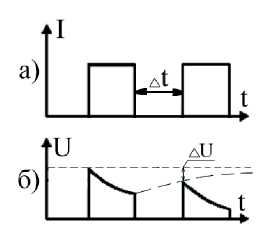
\includegraphics[]{img/9}
	\caption{Метод модуляции проводимости: а) импульсы тока; б) изменение падения напряжения на образце.}
	\label{fig:figure8}
\end{figure}

\begin{figure}[H]
	\centering
	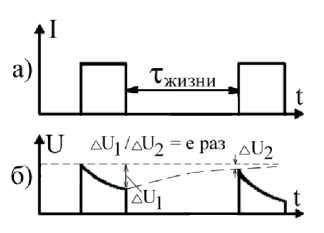
\includegraphics[]{img/10}
	\caption{Зависимость амплитуды второго импульса от времени задержки.}
	\label{fig:figure9}
\end{figure}



Этот закон описывается экспоненциальной функцией времени. Таким образом, зависимость разности амплитуд импульсов напряжения  $U_1-U_2$ от времени задержки, исключая окрестности точки $t = 0$, может быть представлена экспоненциальной функцией вида
\begin{gather}
	\label{eq17}
	U_{1}-U_{2} \sim e^{-t/\tau},
\end{gather}
где $\tau$ -- время жизни неосновных носителей заряда.

Соответственно зависимость $\ln(U_1-U_2)$ от $t$ графически изображается прямой линией, для которой обратное значение тангенса угла наклона равно по абсолютной величине времени жизни.

В данной работе используются точечные контакты, поэтому найдем падение напряжения на распределенном сопротивлении точечного контакта при пропускании через образец импульса постоянного тока $I$. Воспользуемся формулой
\begin{gather}
	\label{eq18}
	U=I R=\frac{\rho l}{S} I
\end{gather}
где $\rho$ -- удельное сопротивление, $l$ -- длина, $S$ -- сечение поверхности, через которую течет ток. 

Заметим, что формула \eqref{eq18} справедлива лишь для проводника с постоянным поперечным сечением $S$, когда линии тока параллельны друг другу. 
В нашем случае линии тока будут расходиться от острия контакта в радиальном направлении. Поэтому роль поперечного сечения будет играть поверхность полусферы переменного радиуса.
\begin{figure}[H]
	\centering
	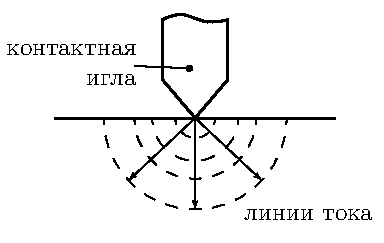
\includegraphics[width = 0.5\linewidth]{fig/curr.pdf}
	\caption{Радиальное растекание тока от точечного контакта}
	\label{fig:figure10}
\end{figure}

Ввиду этого необходимо произвести интегрирование по радиусу по всей области его изменения, то есть от $d$ до $\infty$ ($d$ -- радиус острия контакта). 

Тогда
\begin{gather}
	\label{eq19}
	U(t)=I \int_{d}^{\infty} \frac{\rho(t) \dd l}{2 \pi l^{2}}
\end{gather}

В формуле \eqref{eq19} $U$ не выражается явно как функция времени задержки $t$. Однако, зависимость $U$ от $t$ проявляется через удельное сопротивление, которое является функцией времени задержки.

Как было показано в разделе 1.3, концентрация неосновных носителей заряда изменяется со временем по экспоненциальному закону. Мы можем поэтому представить удельное сопротивление как сумму не зависящего от времени и экспоненциально убывающего слагаемых: 
\begin{gather}
	\label{eq20}
	\rho(t)=\rho_{0}+\rho_{1} e^{-\frac{t}{\tau}}
\end{gather}
где $\tau$ -0 время жизни неосновных носителей заряда.

Предположим, что время задержки между двумя импульсами тока равно $t$. Для этого случая найдем соответствующую разность
импульсов напряжения. Очевидно, что для первого импульса тока время задержки следует считать равным бесконечности, так
как для него $р = р_0$, что выполняется при $t\to\infty$. Поэтому
\begin{gather}
	\label{eq21}
	U_{1}-U_{2}=U(\infty)-U(t)=\frac{I}{2 \pi}\left(\int_{d}^{\infty} \frac{\rho_{0}}{l^{2}} d l-\int_{d}^{\infty} \frac{\rho_{0}-\rho_{1} e^{-\frac{t}{\tau}}}{l^{2}} d l\right)
\end{gather}
В результате получим уравнение вида
\begin{gather}
 	\label{eq22}
 	U_{1}-U_{2}=\left(\frac{I \rho_{1}}{2 \pi} \int_{d}^{\infty} \frac{d l}{l^{2}}\right) e^{-\frac{t}{\tau}},
 \end{gather}
 в котором множитель, стоящий в скобках, является постоянной величиной, не зависящей от времени задержки. Таким образом,
 разность импульсов напряжения со временем меняется по экспоненциальному закону \eqref{eq17}.


Установка включает в себя блок генерации двух импульсов, позволяющий изменять время задержки между импульсами, держатель
с образцом и осциллограф (рис.  \ref{fig:figure11}). Согласно методике, описанной выше, измеряя разность амплитуд
импульсов в зависимости от задержки между ними можно определить время жизни неосновных носителей в образце. Для этого
строится график зависимости логарифма этой разности от времени задержки. По котангенсу угла наклона определяется время
жизни неосновных носителей.
\begin{figure}[H]
	\centering
	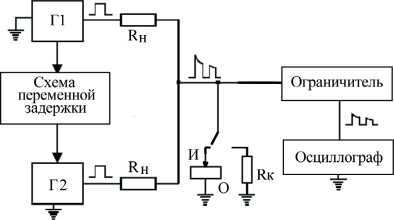
\includegraphics[width = 0.6\linewidth]{img/12}
	\caption{Блок схема установки для измерения времени жизни:
И -- игла, О -- образец, $R_k$ -- калибровочное сопротивление, $R_h$ -- сопротивление нагрузки, Г1 и Г2 -- генераторы напряжения }
	\label{fig:figure11}
\end{figure}
% <img src="Время_жизни_2011_files/1240353c4f_3638373d38_2011-12.jpg" style="width:189pt;height:105pt;"/


\section{Метод измерения диффузионной длины неосновных носителей заряда}

Для определения диффузионной длины используют метод модуляции проводимости полупроводника при импульсном освещении, для
чего применяют светодиод инфракрасного диапазона. Неравновесные носители, генерированные излучением светодиода,
собираются с помощью вольфрамового зонда, служащего коллектором. Результирующий ток подается на сопротивление нагрузки,
напряжение на котором регистрируется с помощью осциллографа.

\begin{figure}[H]
	\centering
	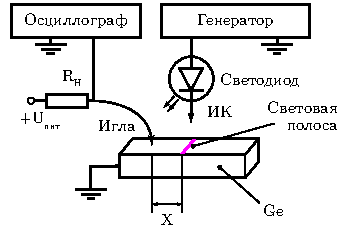
\includegraphics[width = 0.5\linewidth]{fig/scheme.pdf}
	\caption{Блок схема установки для измерения диффузионной длины неосновных носителей заряда}
	\label{fig:figure12}
\end{figure}

% <img src="Время_жизни_2011_files/1240353c4f_3638373d38_2011-13.jpg" style="width:162pt;height:108pt;"/>

Так как коллекторный ток прямо пропорционален концентрации неосновных носителей заряда вблизи точечного контакта, то
можно считать, что падение напряжение на нагрузке прямо пропорционально концентрации дырок. Измеряя напряжение при
различных расстояниях между коллектором и освещенной полосой можно определить диффузионную длину. По сути если световая
полоса отодвинулась от коллектора на расстояние равное диффузионной длине, то амплитуда импульса напряжения изменилась в
$е$ раз. Для более точного определения диффузионной длины строится график зависимости $\ln(U)$ от $x$. Котангенс угла
наклона этой прямой определяет величину диффузионной длины.

Частота импульсов светодиода выбрана так, что во время импульса излучения в образце должно устанавливаться равномерное
распределение неосновных носителей, а за время, когда образец не облучается, неосновные носители должны полностью
рекомбинировать.

\section{Описание экспериментальной установки}

Экспериментальные установки для измерения времени жизни и диффузионной длины собраны в едином приборе, имеющем два режима работы (рис.  \ref{fig:figure13}). При измерении времени жизни вольфрамовая игла служит инжектором носителей. При измерении диффузионной длины генерация носителей осуществляется при помощи облучения, а игла служит коллектором.
\begin{figure}[H]
	\centering
	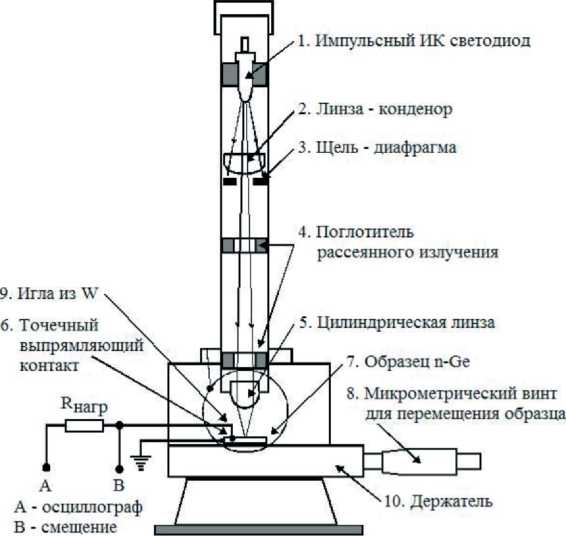
\includegraphics[width = .5\linewidth]{img/14}
	\caption{Конструкция установки для генерации неравновесных носителей в образце.)
}
	\label{fig:figure13}
\end{figure}
% <img src="Время_жизни_2011_files/1240353c4f_3638373d38_2011-14.jpg" style="width:271pt;height:257pt;"/>


Установка состоит из осветителя, в качестве которого используется импульсный светодиод инфракрасного диапазона \textbf{1}, оптической системы \textbf{2-5}, держателя \textbf{10}, в котором крепится образец \textbf{7} и осциллографа. Держатель представляет собой столик с кристаллодержателем, который может перемещаться в горизонтальном направлении. Отсчет продольного перемещения столика производится по микрометрическому винту \textbf{8}. К образцу прижимается вольфрамовый зонд \textbf{9}, служащий коллектором.

Схематический чертеж установки приведен на рисунке \ref{fig:figure13}. Излучение импульсного светодиода инфракрасного диапазона с помощью системы линз, изображенных на рисунке, фокусируется на образце n-Ge в линию шириной $\sim0.1$ мм, которая пересекает всю верхнюю грань образца и параллельна его торцам. Такая система освещения образца упрощает решение задачи диффузии неравновесных носителей, и на известном расстоянии от освещенного участка позволяет свести ее к одномерной задаче, рассмотренной выше.

\newpage
\section*{Эксперимент}

\subsection*{Диффузионная длина}
Определение диффузионной длины неосновных носителей тока. Было произведено измерение амплитуды импульса в мВ в зависимости от
расстояния $x$ между максимальным значением (световым пятном) и щупом.

График зависимости $\ln(U)$ как функции расстояния $x$ приведен на рис. \ref{fig:exp.1}.
\begin{figure}[H]
	\centering
	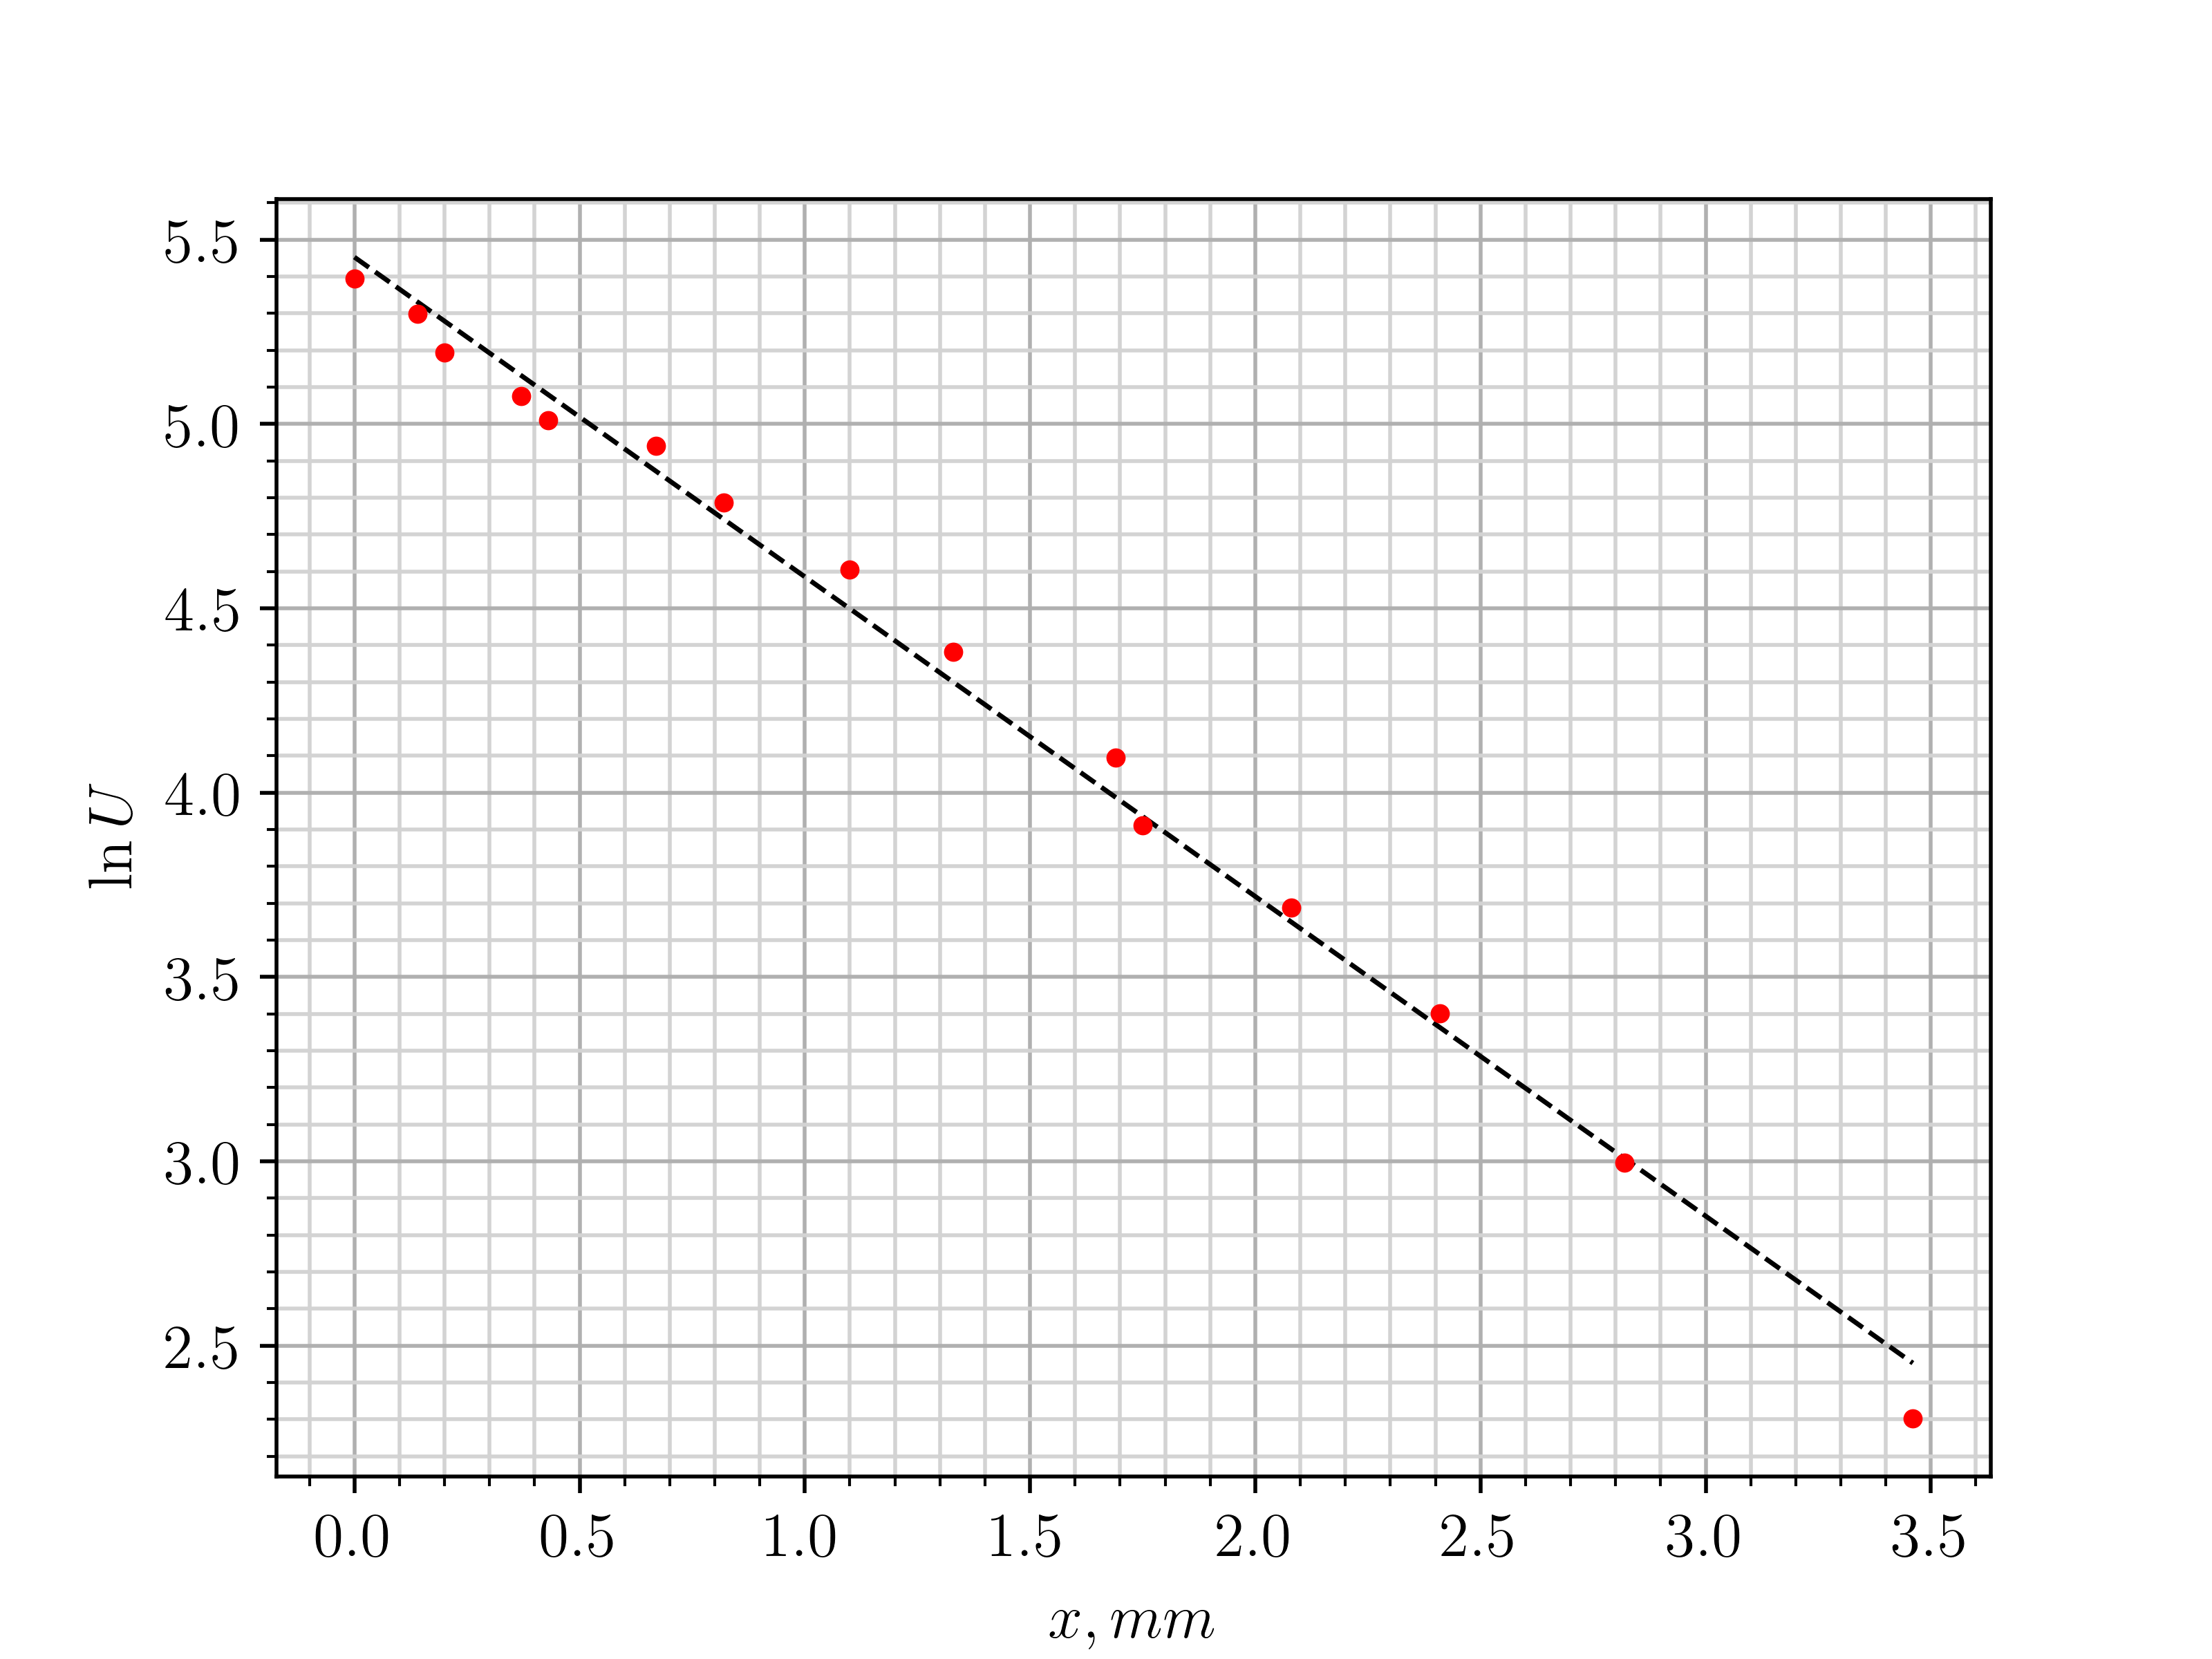
\includegraphics[]{graphs/task1.png}
	\caption{Зависимость логарифма напряжения от расстояния}
	\label{fig:exp.1}
\end{figure}
Амплитуда импульса прямо пропорциональна концентрации неосновных носителей тока. Т.к. $\tan \theta$ прямой соответствует
спадению амплитуды в $e$ раз, то по наклону прямой определили диффузионную длину:
$$\ln U \approx -0.867 x + 5.453,~ r^2 \approx 0.98$$
$$ x_L = \frac{1}{\tan \theta}$$
$$L_p = x_L = 1.2 \pm0.02~mm $$


\subsection*{Время жизни неосновных носителей тока}
Изменяя время задержки между импульсами от 0 до 25 мкс, была измерена зависимость разности амплитуд первого и второго
импульсов от задержки.

Время жизни неосновных носителей определяется как равное времени задержки импульсов, когда напряжение второго импульса
спало в $e$ раз относительно первого. 
$$ U_1 - U_2 \approx e^{-t/\tau}$$ 
$$\Delta U_2 \approx e^{-t/\tau} \Rightarrow \ln(\Delta U_2) \approx \frac{-t}{\tau}$$   
\begin{figure}[H]
	\centering
	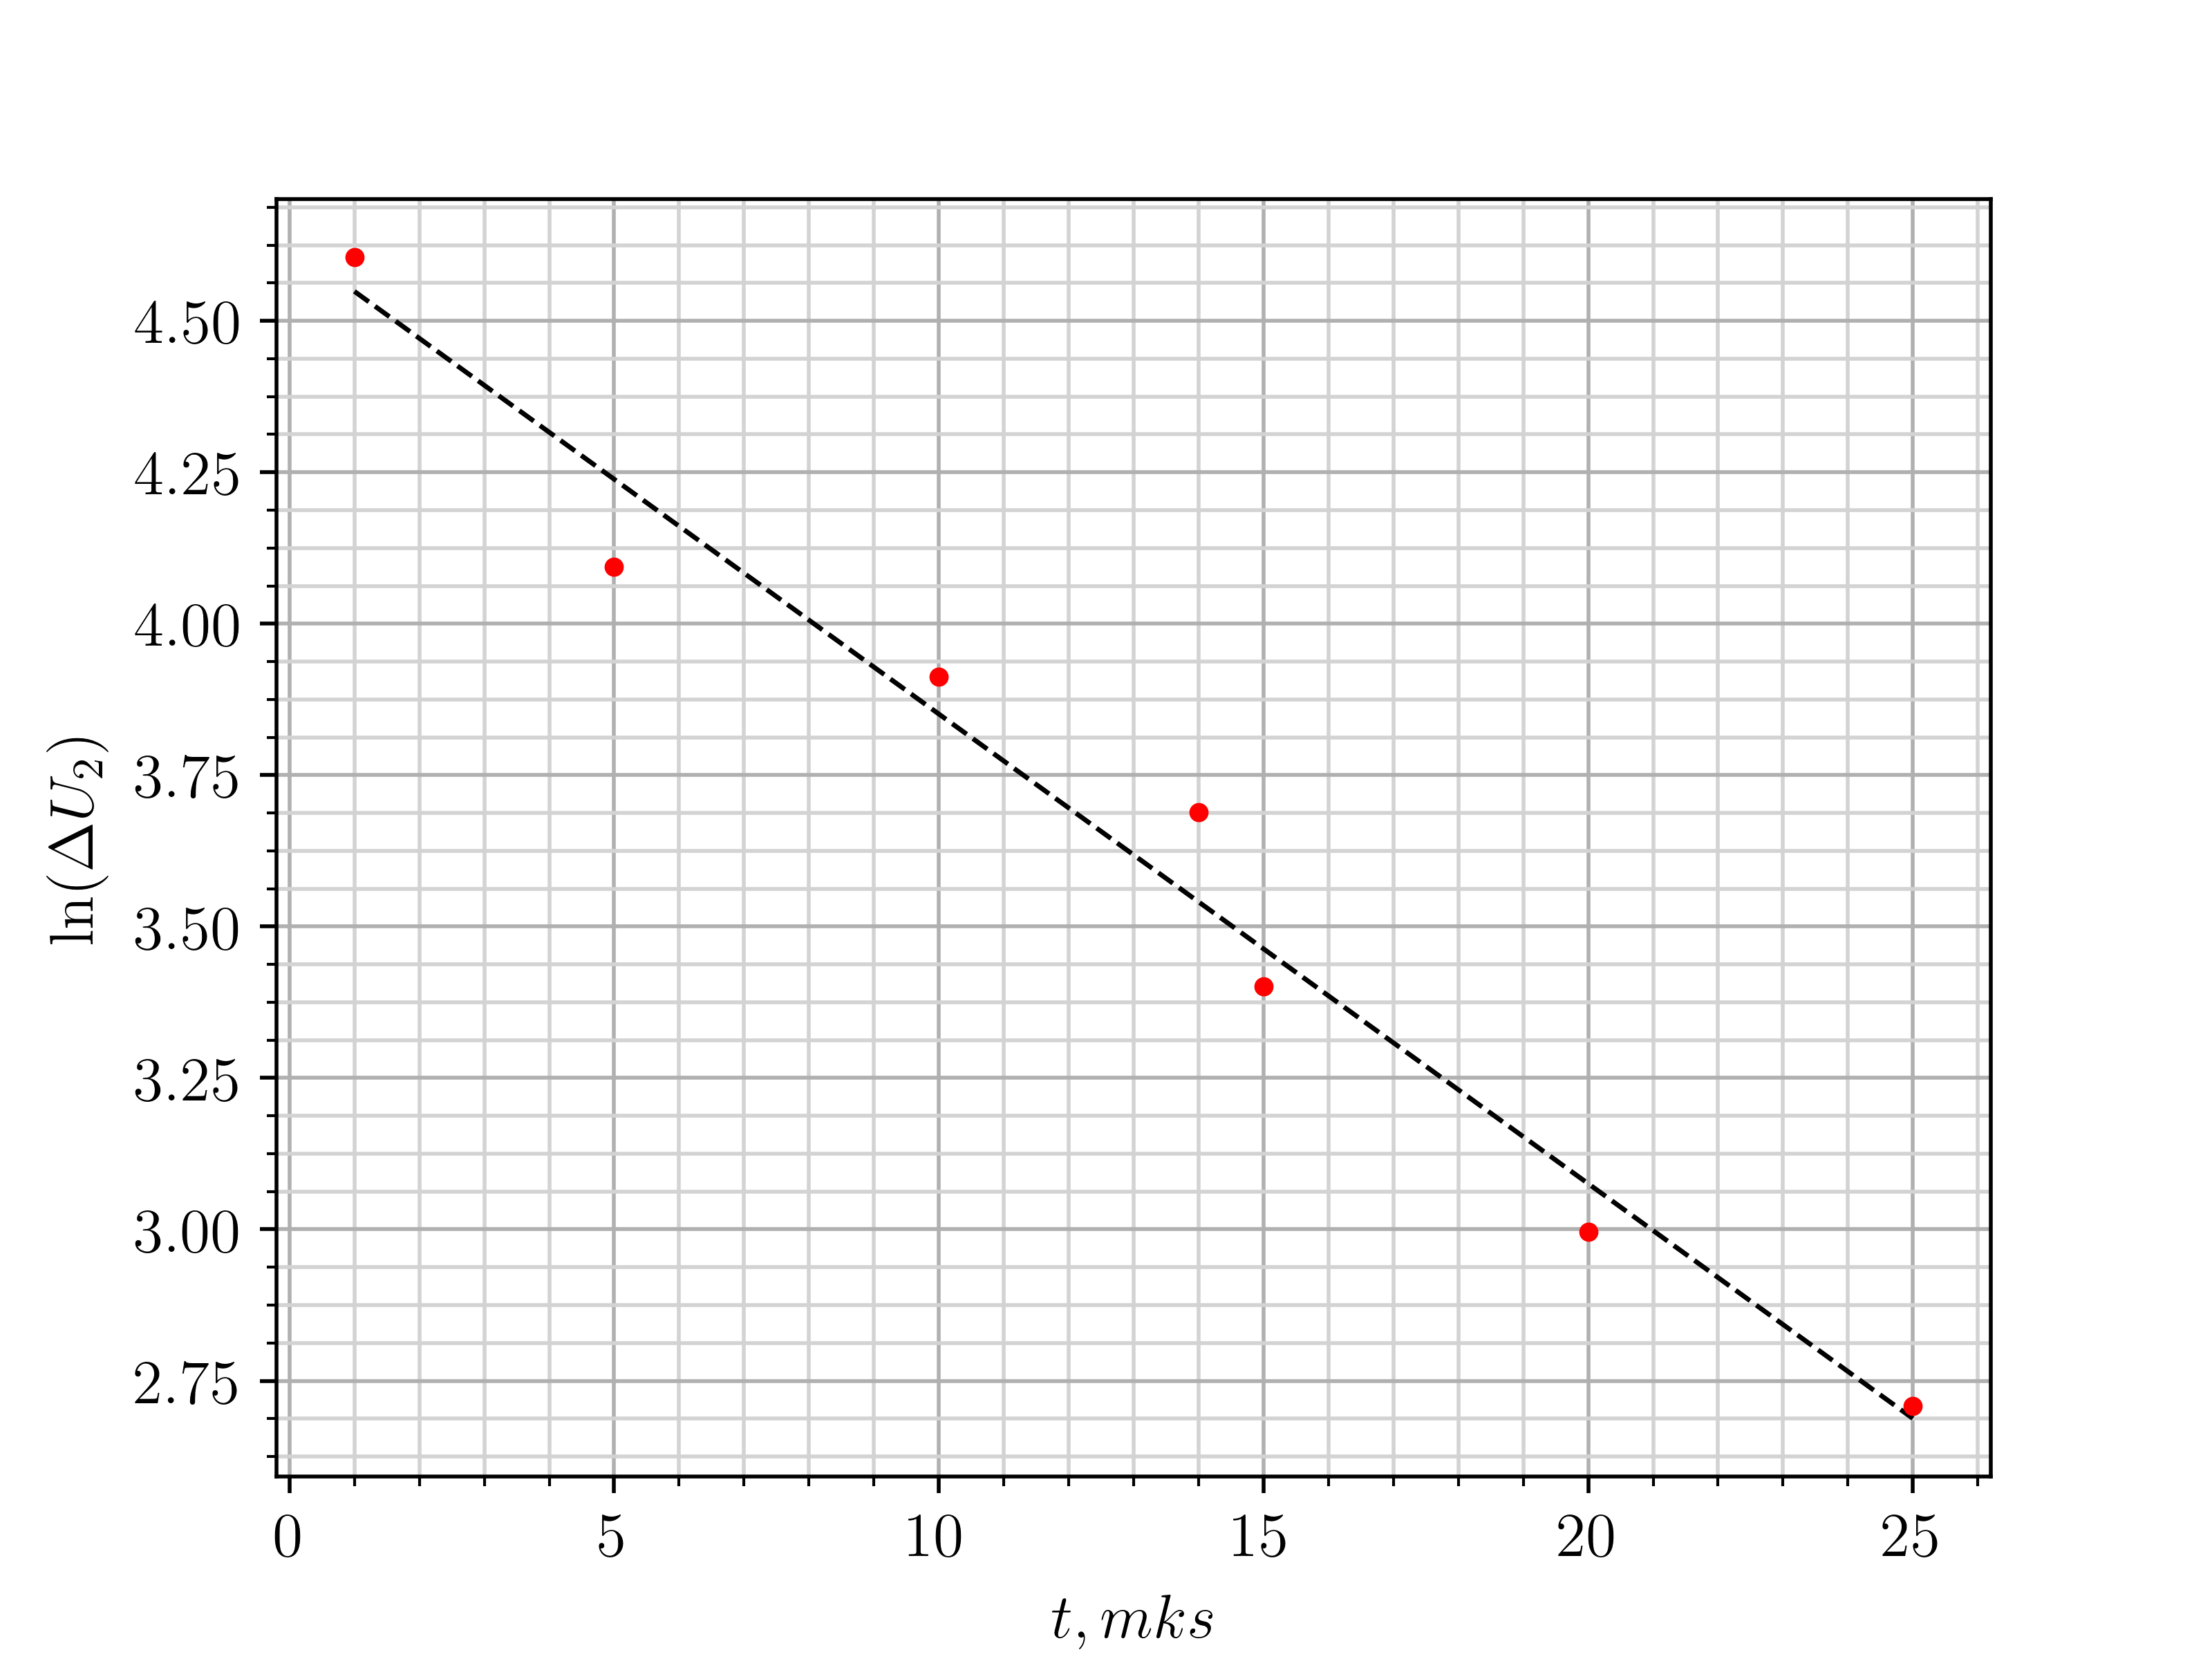
\includegraphics[width=.8\linewidth]{graphs/task2.png}
	\caption{Зависимость логарифма разности амплитуды напряжения от времени задержки. Коэффициент детерминации $r^2 \approx 0.98$}
	\label{fig:exp.2}
\end{figure}
Полученное значение для наклона прямой $\tan \theta \approx -0.0775 $. Тогда время жизни неосновных носителей:
$$\tau_L = \frac{1}{-\tan \theta} $$
$$ \tau_L = 12.9 \pm 0.3~mks $$

\section*{Итоги}
В данной работе была определена диффузионная длина, а так же время жизни неосновных носителей тока в исследуемом
образце:
\begin{itemize}
	\item $L_p = 1.2\pm0.02~mm$
	\item $\tau_L = 12.9\pm 0.3~mks$
\end{itemize} 

\end{document}